\chapter{提案手法}

\section{概要}
本章では、本研究で提案するシステムについて説明する。
本研究では、識別精度を犠牲にすることなくアノテーションコストを最小化する病理画像解析のための深層能動学習システムを構築する。
高精度を達成するために識別器にConvolutional Neural Networkを採用し、少ないラベル数でも学習を収束させるために
ImageNetで学習済みのpretrained-networkの重みからfinetuneして学習を行う。
一般画像認識のために学習されたモデルでも、医療画像解析への転移学習は幅広いタスクに対して有効であると知られているため、妥当であると考えられる。

また、前章で述べた深層学習と能動学習の組み合わせの問題に対する解決するためのアプローチとして、Query-By-Dropout-Predictionsを提案する。
不確かさを定義しない多層ニューラルネットワークを効率的にパラメータを更新するためのサンプルを見つけるために、予測時にもDropuotを利用するアプローチである。
さらに、医療画像解析において重要であると考えられる様々な変形に対する不変性の担保を考慮し、
各Committeeのprediction時にもランダムなData Augmentationを利用することで、識別に有効なサンプルのみではなく
不変性を確保するために有効であるサンプルをクエリとして選択することを考える。
また、能動学習において一般に問題となるサンプリングバイアスを解決するためにクラスタリング手法を採用し、
その際に用いる特徴量について妥当だと考えられるものを実験から選定した。

以下の節では、それぞれについて詳細を説明する。

\clearpage

\begin{figure}[tbp]
    \label{fig:overview}
     \begin{center}
      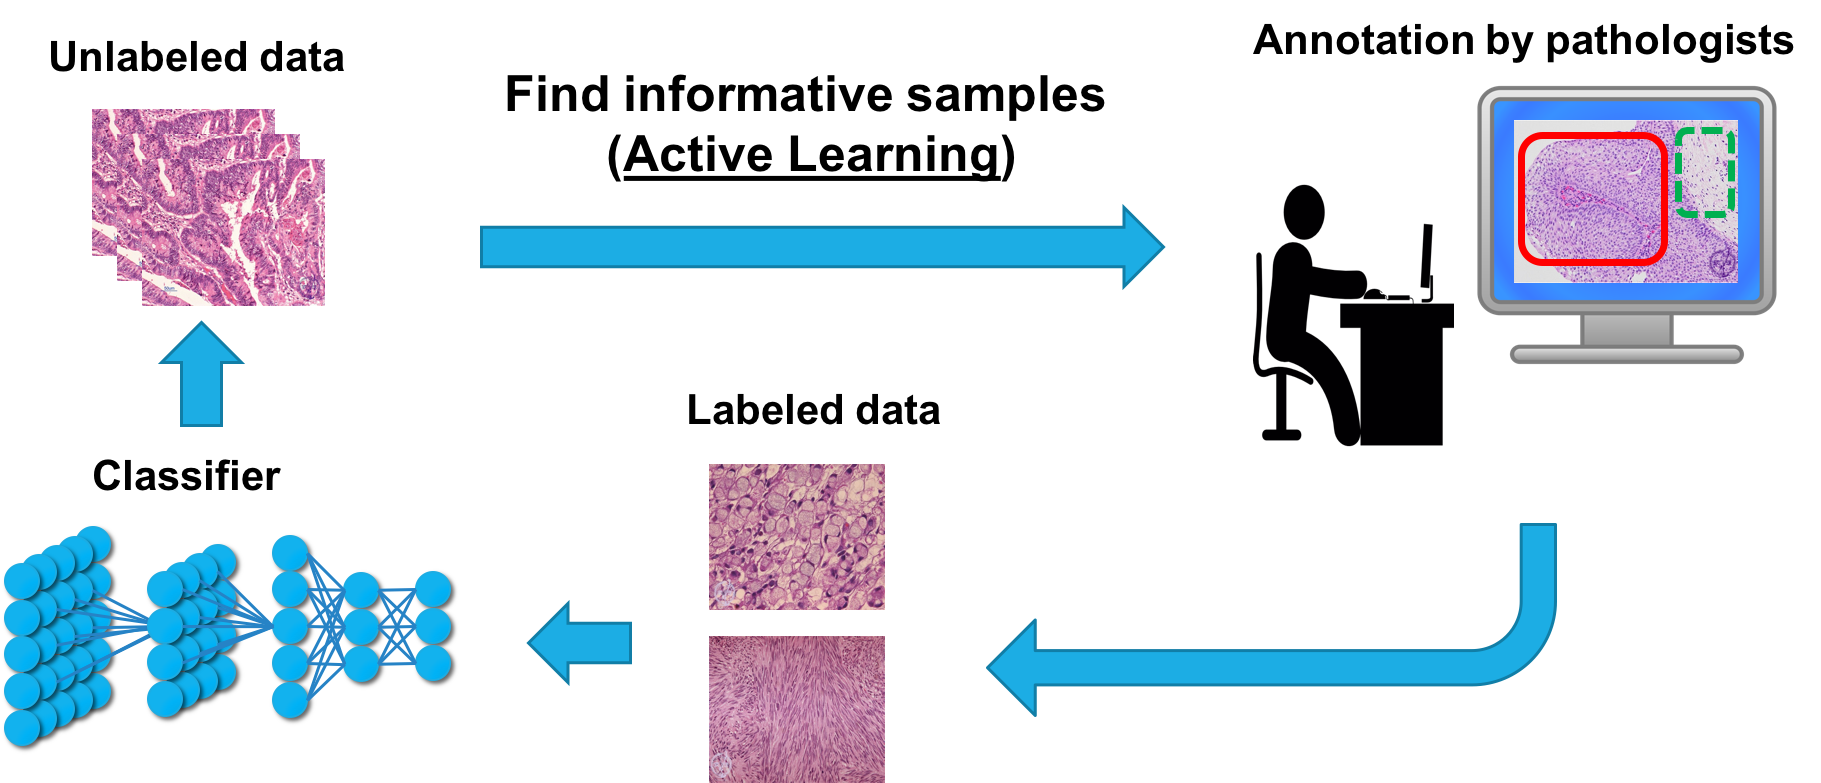
\includegraphics[width=120mm]{figures/overview.png}
     \end{center}
    \caption{本研究で提案するシステムの概念図}
\end{figure}

\section{Query by Dropout predictions}
多層ニューラルネットワークによって識別問題を解く際には、最終出力が各ラベルに対応する確率となる確率分布となるように設計して学習を行う。
多層ニューラルネットワークを能動学習に利用する際にはこの確率分布のエントロピーの大きさなどを利用して不確かさを定量評価し、
Uncertainty Samplingによってクエリ選択を行う。
しかし、前章で述べたように、ニューラルネットワーク自体のパラメータに対する不確かさをモデルしているわけではない。
このように不確かさを陽にモデル化しない識別器を利用した能動学習においては、
バージョン空間を近似的に保持することで有効なサンプルを選択するQuery By Committeeを用いる事が多いが、
多層ニューラルネットワークのように非常に計算コストの重いモデルを複数同時に保持し学習を行うことはメモリ、
計算時間等様々な問題で現実的ではないという問題があった。
そこで、本研究では、多くの深層学習のアーキテクチャで正則化の目的で利用されるDropoutによって、
本体のネットワークからサンプリングされた部分ネットワークをCommitteeとみなし、
それらの予測の不一致度を利用して近似的にQuery-By-Committeeを行う手法を提案する(Fig.\ref{fig:query_by_dropout})。
これらの部分ネットワークがCommitteeとして利用されるためには、それらが訓練データに対してはConsistentであり、
かつ、それぞれの未知データに対する出力には分散を持つ必要がある。
この性質について実験で検証し、Uncertainty Samplingのみを利用する方法と比較する。

\begin{figure}[tbp]
    \label{fig:query_by_dropout}
     \begin{center}
      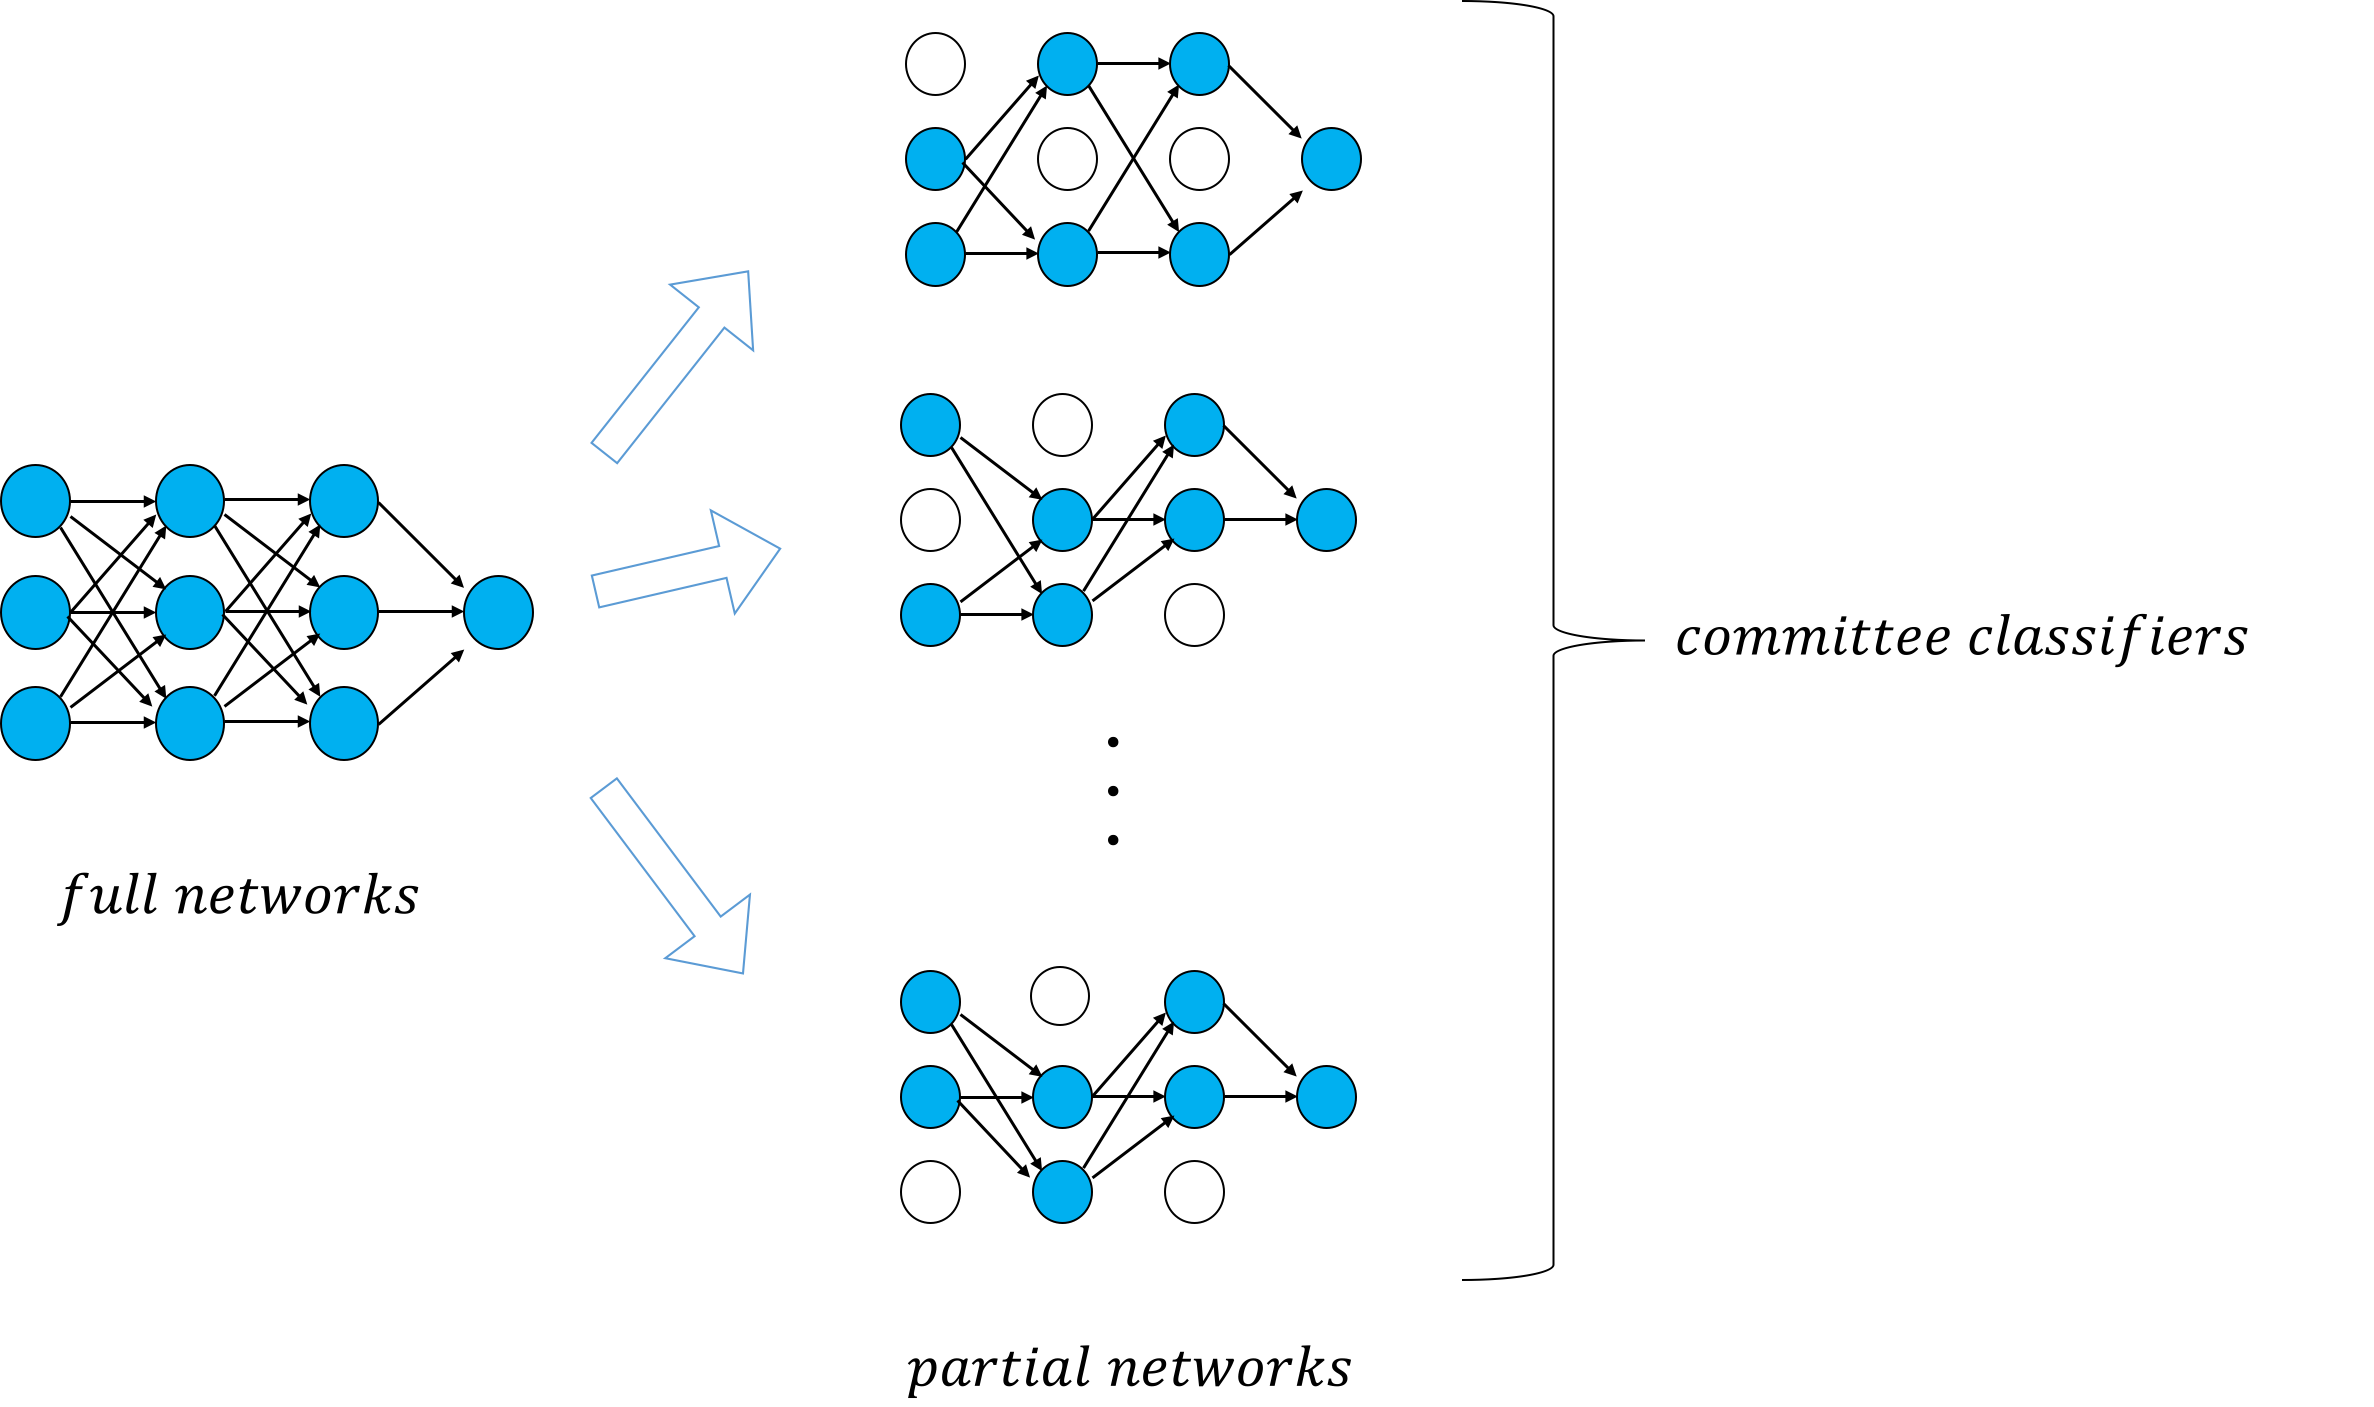
\includegraphics[width=120mm]{figures/query_by_dropout.png}
     \end{center}
    \caption{Dropoutによってサンプリングされた部分ネットワークによってCommitteeを形成する。}
\end{figure}

\section{推論時でのData Augmentationの利用}
医療画像解析では、一般画像認識と比較してモデルが獲得すべき不変性が多く存在する。
多くの研究では、訓練時に画像に対してData Augmentationを利用することで不変性を獲得させる。\todo{日本語やべえ}
また、ラベル付きデータが少ない場合には特に有効であると知られており、本研究でも、識別器を学習させる際には採用する。
上記でDropoutによって部分ネットワークCommitteeを生成することで不一致度を図る手法を提案した。
本研究ではそれだけではなく、Data Augmentationを推論時も利用することで

\section{提案手法の動作原理}
pre-trained networkを利用する。
基本的にはdropoutはfully connected層で行う
よってそれらは識別境界を大きく変更させるためのサンプルを取得することができる。
Data augmentationを利用することで

\section{バッチ型能動学習への拡張}
能動学習では、クエリ問い合わせを行いラベルデータを拡充するごとに、識別器をfrom scracthから学習させるのが一般的である。
深層学習器を能動学習に利用する場合、一度の再学習に大きな計算コストがかかってしまうため、
各クエリ問い合わせにおいて複数のサンプルにラベリングを付与してもらうバッチ型能動学習を採用するのが適当であると考えられる。
一度に投げるクエリ内で情報の重複が起きないようにするためには何らかの工夫をする必要があるが、
2章で述べたような劣モジュラ関数を設計するのは深層学習を利用する場合計算コストの観点から難しい。
そこで、本研究ではクラスタリングにより同一のクラスターに属するサンプルは2つ以上選択しないとすることで、情報の重複を避ける。
また、クラスタリングに使用する特徴量の候補として、以下の3つを考慮した。

\subsubsection{hand-crafted feature}
2章で述べたように、病理画像解析にはテクスチャ解析で用いられる技術がしばしば使用される。
ここでは、パターンベースの特徴量で、位置不変性と輝度変化への頑健性を有するLocal Binary Pattern (LBP)を採用する。
実際には、回転不変性を担保させるようにLBPを改良したimproved LBPを利用した。

\subsubsection{CNNの中間特徴量}
Imagenetで学習された特徴量は様々なタスクに有用であるとされており、多数の医療画像解析で利用されている。
本研究ではGoogleNetの中間特徴量を利用した。

\subsubsection{compact bilinear poolingによる特徴量}
近年の深層学習を用いたテクスチャ解析の研究で、Bilinear Poolingによって空間情報をなくした特徴量がしばしば利用される。
これは、CNNの中間特徴量の相関行列を計算し空間方向に平均を取ったものである。
\begin{eqnarray}
G_{ij} = \sum_k{F_{ik} F_{jk}}
\end{eqnarray}
また、一般にCNNの特徴量次元(チャンネル数)は256~512の大きな値であるため、そのまま計算した場合非常に高次元な値となってしまう。
そこで、その近似手法であるCompact Bilinear Pooling\cite{gao2016compact}を本研究ではCNNを用いたテクスチャ特徴量として採用する。

\section{アルゴリズムの流れ}
以上で述べたそれぞれの手法をまとめる



